\subsection{Overview}
\graphicspath{ {./texfiles/electrical/eimc/} }
%Electrical overview content here

\subsubsection*{Main requirements and design constraints}
Our high-voltage battery is required to 
\begin{itemize}
    \item power the EMRAX 188 MV motor, requiring a maximum of 120 A at 504 V for full power, through the traction inverter
    \item endure multiple runs 
    \item fit into the chassis appropriately
    \item do not exceed a weight limit of 30kg, also considering the efforts to remove it. Therefore, high energy (and power) density were important, removing the option of lead-acid batteries that are used in the railway sector. The high current ratings made specialized Lithium-Polymer cells one of the few, and the cheapest option available, which was to consider given the limited funds we had.
    \item be reliable and tested: The team designing the batteries originally come from a diverse background, having experience with manufacturing lithium battery packs. However, experimental innovative designs like supercapacitors or sodium ion cells were not feasible in the time. 
    \item be easily removable for maintenance
    \item be controlled by a battery management system, due to obvious safety reasons
    \item life cycle of at least 3 years for financial and environmental sustainability.
    \item have power headroom for future designs, being able to be reused. We therefore also ordered a surplus of 30 cells.
    \item cost less than 5000€, as a fund of a local bank is sponsoring us with 5000€ for the battery system (including BMS).
    \item charge at a rate of approximately 1C for time constraints.
    \item not heat up excessively, as we only opted for passive cooling.
\end{itemize}
The main design requirement was to satisfy the motor's needs, which are as follows:
\begin{figure}[H]
    \centering
    \includegraphics[page=2,width=\textwidth]{texfiles/mech/eimg/propulsion/table_motor}
    \caption{Motor Specifications}
    \label{fig: Motor Specifications}
\end{figure}

The maximum voltage ratings have been increased several times in the past two years by the manufacturer, allowing for higher voltages. However, we stick to the initial data that we were given in the previous design. We will not reach the level that the motor is tested at (>800V DC maximum voltage). \\
\subsection{Electrical and mechanical design process}
%Electrical and mechanical design process content here
Our design followed these steps.\\
\begin{wrapfigure}{r}{0.25\textwidth}
    \centering
    \includegraphics[width=0.25\textwidth]{texfiles/elec/eimg/BatteryDesignProcess}
    \caption{Heuristic for Finding Battery Parameter}
\end{wrapfigure}
For easier simulations, we used a matlab script with different parameters, which is publicly accessible via Github \footnote{\href{https://github.com/Team-Tachyon-e-V/battery_model}{Link to our battery model estimation}}:
\subsubsection*{Pod Characteristics} 
Some constant mechanical coefficients for the pod's movement that we assumed in our calculations:

\begin{align*}
m_{\text{fzg}} &= 250 \, \text{kg} & \text{(Vehicle Mass)} \\
m_{\text{zul}} &= 50 \, \text{kg} & \text{(Payload)} \\
c_L &= 0.8 & \text{(Drag Coefficient)} \\
\rho_L &= 1.2 \, \text{kg/m}^3 & \text{(Air Density)} \\
f_r &= 0.02 & \text{(Kinetic Friction Coefficient)} \\
g &= 9.81 \, \text{m/s}^2 & \text{(Gravitational Acceleration)} \\
A &= 1.5 \times 0.3 \, \text{m}^2 & \text{(Frontal Area)} \\
e_{i1} &= 1.2 & \text{(Mass Factor for Rotating Part)} \\
\text{Gradient} &= 5\% & \text{(Inclination Gradient Percentage)} \\
\alpha &= \arctan\left(\frac{\text{Gradient}}{100}\right) & \text{(Inclination Gradient Angle)}
\end{align*}

\subsubsection*{Mass Calculation}

Effective mass that will be accelerated:

\begin{align*}
m_{\text{acc}} =  e_{i1} \times m_{\text{fzg}} + m_{\text{zul}} = 1.2 \times 300 \, \text{kg} = 360 \, \text{kg}
\end{align*}

\subsubsection*{Vehicle Dynamics Parameters}

Parameters related to the pod's movement:

\begin{align*}
v_{\text{init}} &= 0 \, \text{m/s} & \text{(Starting Velocity)} \\
v_{\text{max}} &= \frac{60}{3.6} \, \text{m/s} \approx 16.67 \, \text{m/s} & \text{(Maximum Velocity)} \\
s_f &= 150 \, \text{m} & \text{(Pod Distance)} \\
R_d &= 0.1 \, \text{m} & \text{(Radius of Driving Wheel)} %should be diameter
\end{align*}

\subsubsection*{Motor Parameters}

Motor's specifications:

\begin{align*}
P_{\text{peak}} &= 37 \times 1000 \, \text{W} & \text{(Power at 7000 rpm)} \\
\text{eff} &= 0.96 & \text{(Efficiency)} \\
P_{\text{motor}} &= 0.96 \times 37000 \, \text{W} = 35520 \, \text{W}
\end{align*}

\subsubsection*{Resistance Calculation for Continuous Power}

We add all resistive forces against the pod's motion, taking into account that we drive in a non-vacuum environment:

\begin{align*}
F_{\text{roll}} &= 0.02 \times 300 \times 9.81 \times \cos\left(\arctan\left(\frac{5}{100}\right)\right) \\
F_{\text{luft}} &= 0.5 \times 0.8 \times 1.2 \times (1.5 \times 0.3) \times (16.67^2) \\
F_{\text{st}} &= 300 \times 9.81 \times \sin\left(\arctan\left(\frac{5}{100}\right)\right)
\end{align*}

\subsubsection*{Maximum Acceleration Calculation}

Pod's maximum acceleration:

\begin{align*}
a_{\text{max}} = \frac{\left(\frac{35520}{16.67}\right) - F_{\text{roll}} - F_{\text{luft}} - F_{\text{st}}}{360}
\end{align*}

\subsubsection*{S-Curve Generation}

Timing for acceleration and deceleration phases:

\begin{align*}
T &= \left(\frac{a_{\text{max}}}{j_{\text{max}}}\right) + \left(\frac{16.67}{a_{\text{max}}}\right) + \left(\frac{150}{16.67}\right)
\end{align*}

\subsubsection*{Energy Demand}

Energy demand for the journey: \text{energy\_bed\_wh} = \text{Energy demand in Wh}

\subsubsection*{Battery Parameters}
%% Voltage and Current Need(from data sheet)

\begin{align*}
V_{\text{bed}} &= 490 \, \text{V}; \\
I_{\text{bed}} &= 100 \, \text{A}; \\
%% Battery Parameters
U_{\text{zell}} &= 4.2 \, \text{V}; \\
C_{\text{zell\_ah}} &= 6.1 \, \text{Ah}; \\
C_{\text{rate}} &= 35; \\
\text{SoC\_max} &= 80\%; \\
\text{SoC\_min} &= 40\%; \\
\textbf{Required battery configuration:}; \\
n_{\text{ser}} &= \left\lceil \frac{V_{\text{bed}}}{U_{\text{zell}}} \right\rceil; \\
C_{\text{tot}} &= \frac{\text{energy\_bed\_wh}}{n_{\text{ser}} \times U_{\text{zell}} \times \text{eff\_mech}}; \\
n_{\text{par}} &= \left\lceil \frac{C_{\text{tot}}}{C_{\text{zell\_ah}} \times \left(\frac{\text{SoC\_max} - \text{SoC\_min}}{100}\right)} \right\rceil; % Add semicolon at the end
\end{align*}
The S-curves are simple, as follows:
\begin{figure}[H]
    \centering
    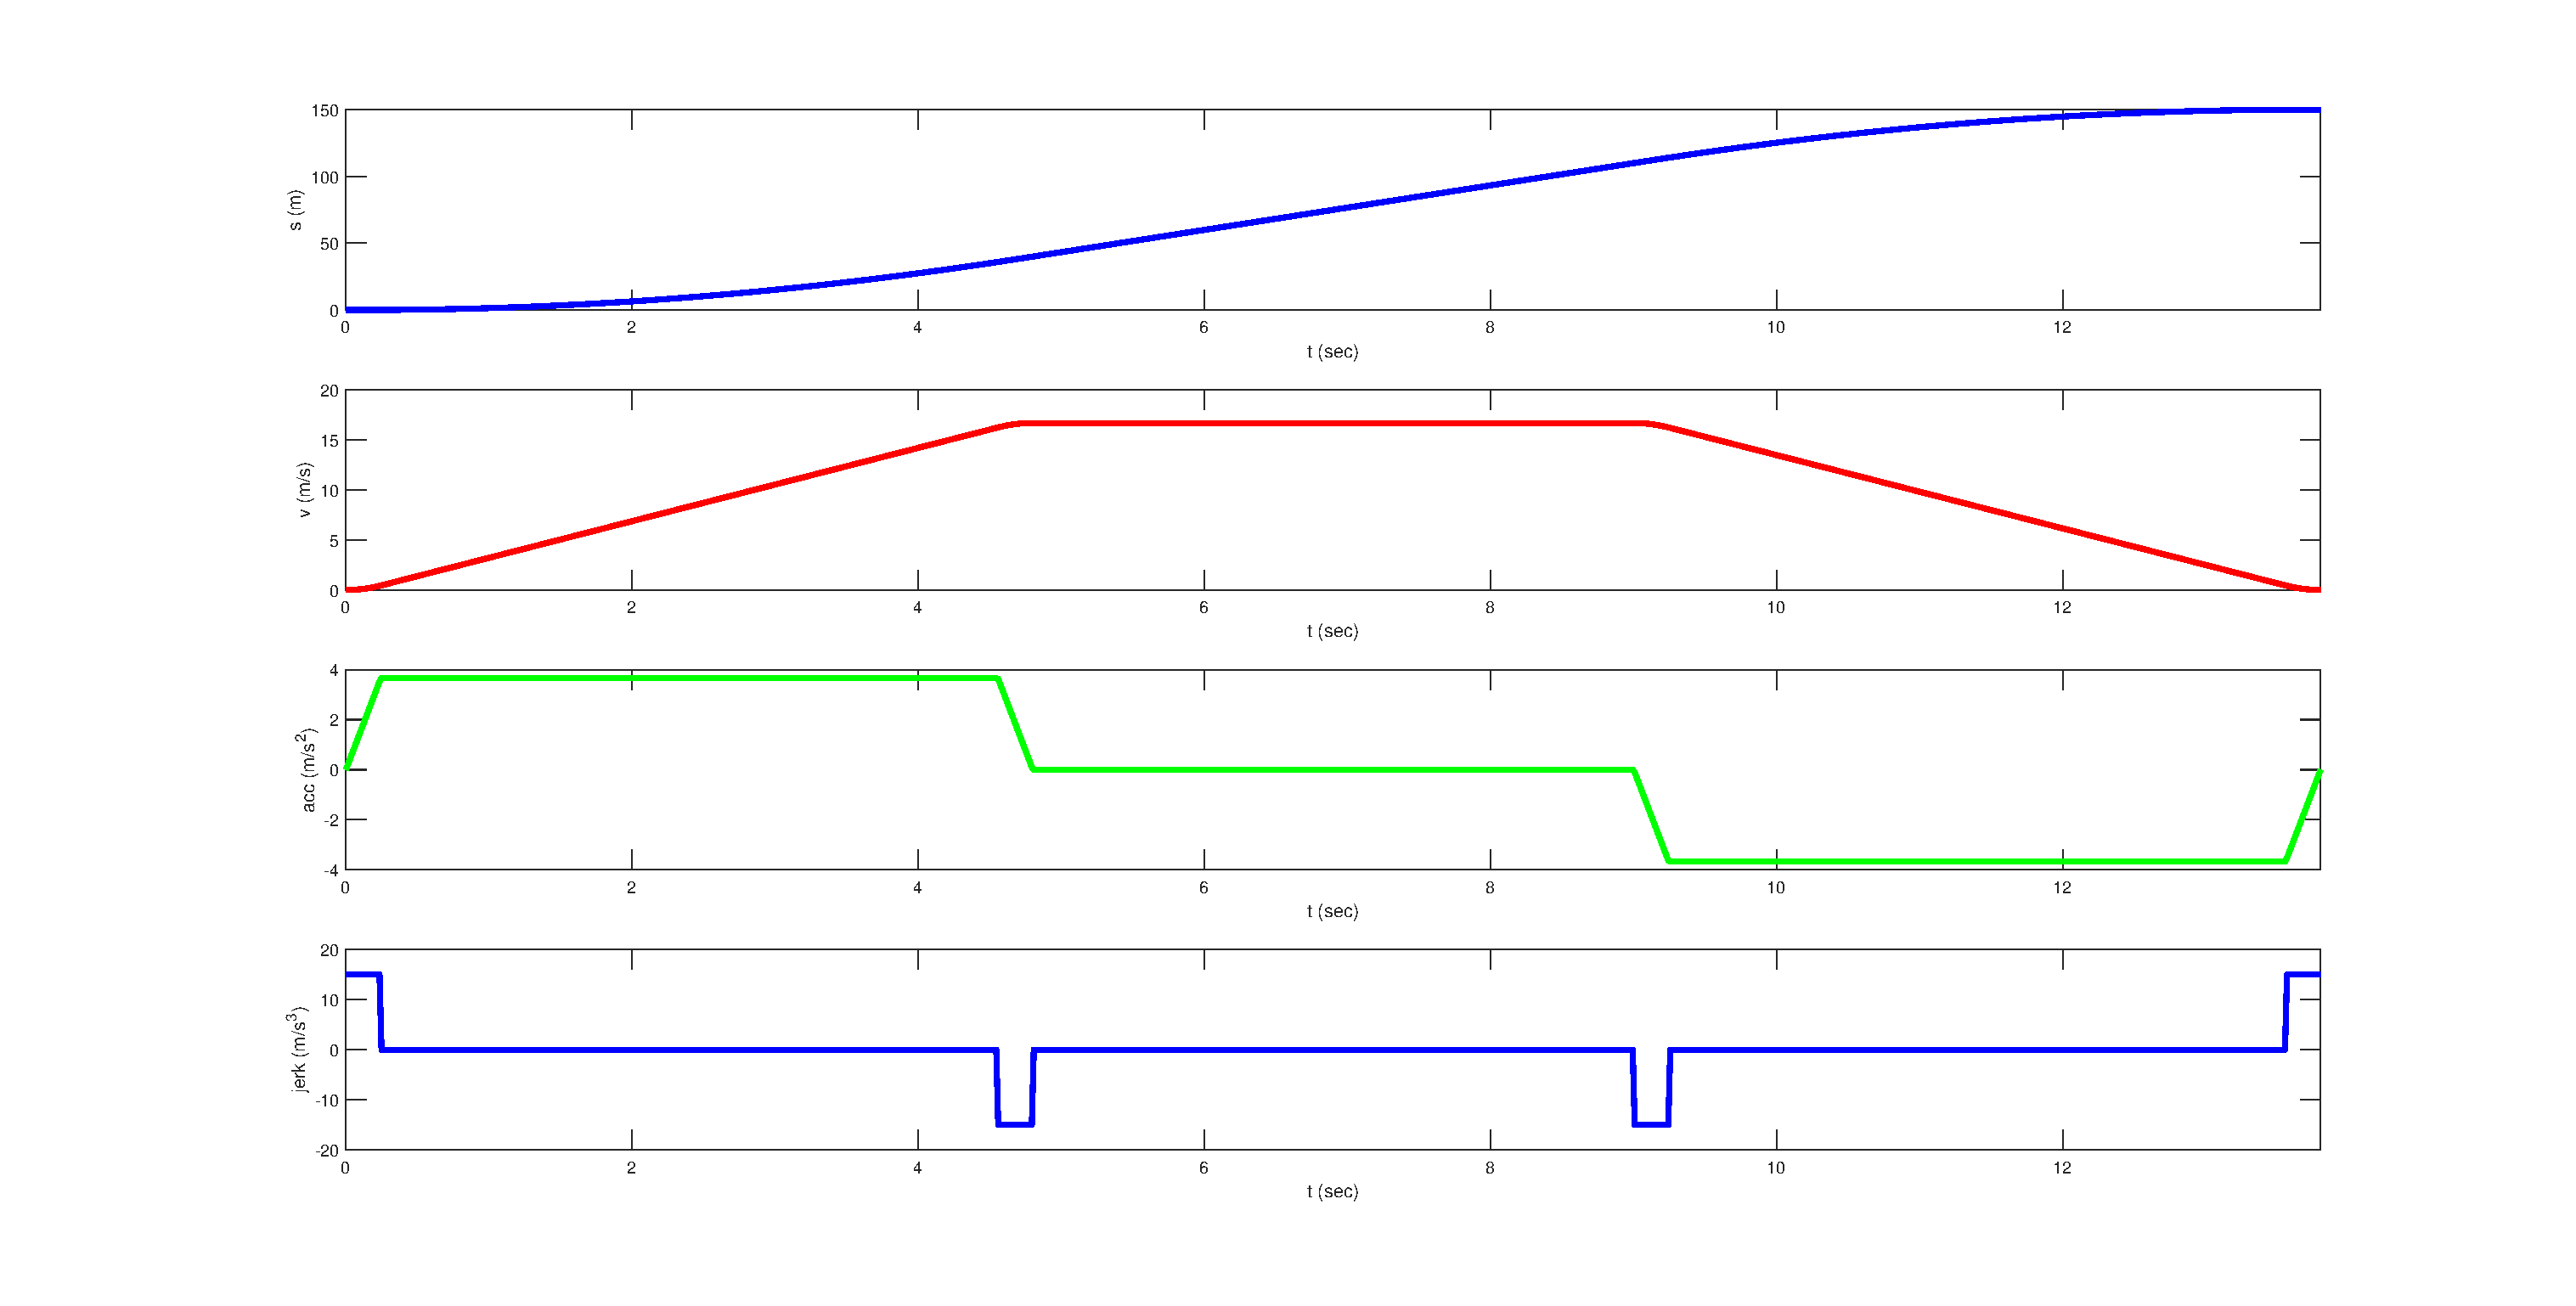
\includegraphics[width=0.9\textwidth]{texfiles/elec/eimg/battery_run_model}
    \caption{Run model}
    \label{img: runmodel}
\end{figure}
The results showed that we needed 117 x 1 cells in series, which can be explained because we assumed to be able to use the maximum voltage, not the nominal voltage of the battery cells. We are able to run 27.47 runs, even with keeping our state of charge between 40 and 80 percent, saving battery health \footnote{We follow general advice that the optimal SOC lay between 0.2 to 0.8, and exceeding this range is not per se damaging to the battery, but shortening its life span, which we try to avoid}.

\subsubsection{Schematics and drawings.}
The battery cell is in a standard pouch format. It has bigger tabs, presumably because of the high currents.
\begin{figure}[H]
    \centering
    \includegraphics[width=0.9\textwidth]{texfiles/elec/eimg/BatteryCell}
    \caption{Battery cell}
    \label{img: Batterycell}
\end{figure}

The CAD models of the battery pack are shown in the following. We visually cut the box open to show the inside structure. For the embedding of the battery pack in its surrounding, please refer to the \ref{sec:chassis}. \\

\begin{figure}[H]
    \centering
    \begin{subfigure}[b]{0.45\textwidth}
        \centering
        \includegraphics[width=\textwidth]{texfiles/elec/eimg/BatteryAssemblyDiag}
        \caption{Battery pack (cut open)}
        \label{img: Batterypack}
    \end{subfigure}
    \hfill
    \begin{subfigure}[b]{0.45\textwidth}
        \centering
        \rotatebox{180}{\includegraphics[width=\textwidth]{texfiles/elec/eimg/BatteryAssemblySide}}
        \caption{Battery pack from the side.}
        \label{img: Battery pack from the side}
    \end{subfigure}
    
    \vspace{1cm}
    
    \begin{subfigure}[b]{0.8\textwidth}
        \centering
        \rotatebox{90}{\includegraphics[width=\textwidth]{texfiles/elec/eimg/BatteryAssemblyTop}}
        \caption{Battery pack from the top}
        \label{img: Battery pack from the top}
    \end{subfigure}
    \caption{Battery pack schematics and drawings}
    \label{img: Battery pack schematics}
\end{figure}

\begin{figure}[H]
    \centering
    \includegraphics[width=\textwidth]{texfiles/elec/eimg/BatteryCableScheme}
    \caption{Schematic of battery pack}
    \label{img: batterycabling}
\end{figure}
\subsubsection{Temperature simulations for vacuum conditions.}
For our heat simulations, we used the software of ANSYS. By vacuum conditions, we assumed the
lack of gas flow, which eliminates the cooling heat flow from winds. The simulation tool solves
the heat transfer equation \( \frac{\partial T}{\partial t} = \alpha \left( \frac{\partial^2 T}{\partial x^2} + \frac{\partial^2 T}{\partial y^2} + \frac{\partial^2 T}{\partial z^2} \right) \)
by discretizing through Finite-Element-Methods. \\
Its results:
\begin{figure}[H]
    \centering
    \includegraphics[width=0.9\textwidth]{texfiles/elec/eimg/SimulationTemplate}
    \caption{Simulation results (MUSTER)}
    \label{img: simresults_battery}
\end{figure}

\subsection{Electrical system characteristics}
%Content of the electrical system characteristics here

\subsection{Interface with other system}
%Interface with other system content here n
\subsubsection{Control systems of the boards}
We configure the BMS prior to the competition, and do not plan to change any settings during the competition. It sends telemetry data over CAN and permits charging/discharging of the battery. \\
All the electric subsystems are located within the pod. \\

The physical connection matrix is as following:
\begin{table}[H]
    \centering
    \begin{adjustbox}{width=\textwidth,center}
    \begin{tabular}{|c|c|c|c|c|c|c|}
    \hline
    From | To & \text{LV Battery} & \text{HV Battery} & \text{BMS} & \text{Traction Inverter} & \text{Motor} & \text{Cooling System} \\
    \hline
    \text{LV Battery} & - & - & Powers & \text{Powers control system} & - & \text{Powers pump and control system} \\
    \hline
    \text{HV Battery} & - & - & Connects to & \text{Provides power} & - & - \\
    \hline
    \text{BMS} & - & - & \text{Controls} & - & - & - \\
    \text{Traction Inverter} & - & - & - & - & \text{Propels} & X \\
    \hline
    \text{Motor} & - & - & - & - & - & - \\
    \hline
    \text{Cooling System} & - & - & - & \text{Cooling} & \text{Cooling} & \text{Cooling (implicitly)} \\
    \hline
    \end{tabular}
\end{adjustbox}
\caption{Physical connection matrix}
\label{Physical connection matrix Battery}
\end{table}

The data connection matrix is as following. All communication between boards are via CAN, if not specified otherwise:

\begin{table}[H]
    \centering
    \begin{adjustbox}{width=\textwidth,center}
    \begin{tabular}{|l|c|c|c|c|c|c|c|c|}
    \hline
    From $\backslash$ To & LV Battery & HV Battery & BMS & Traction Inverter & Motor & Cooling System & Brakes Controller & Telemetry Unit  \\
    \hline
    LV Battery & - & - & - & - & - & - & - & - \\
    HV Battery  & - & - & Discharge rate, voltage level & - & - & - & - & - \\
    BMS & controls & controls & - & - & - & - & - & sends data \\
    Traction Inverter & - & - & - & - & - & - & - & sends data \\
    Motor & - & - & - & - & - & - & - & - \\
    Cooling System & - & - & - & - & - & - & - & sends data \\
    Brakes Controller & - & - & - & - & - & - & - & sends data \\
    Telemetry Unit & - & - & updates limits & sends commands & - & sends target rates & sends commands & - \\
    \hline
    \end{tabular}
    \end{adjustbox}
    \caption{Data connection matrix}
    \label{data-connectivity-matrix-battery}
\end{table}


\subsection{Final system description}
%Description of the system here
\subsubsection{Battery Cells} 

High Voltage Network: \\
Our high voltage battery will make use of lithium-ion polymer technology. We use 120 pouch-format cells from Shenzhen GrePow Battery Co. Ltd rated at 45C maximum discharge that we plan to connect in series. 
The finished package (main battery pack) will be assembled by the team, helped by the ISEA institute of RWTH Aachen University.
We are going to connect the 120 cells connected in series and that will have 1 parallel line. This will roughly have 504 Volt at max (using \(120 * 4.2V = 504 V \) ) 
which provides sufficient electricity to power the motor.
The battery pack will provide up to ~350 Amps of DC current available to the inverter. However, neither the inverter nor the motor is not rated for such high currents nominally, and we are not trying to use the full power of the battery pack.
\newline
Therefore, the maximum output current of the HV Battery will be rated at 120 A maximum (peak) and 74 A continuous. As the peak duration is at 120s, and our runs are at most 10s, we will set the limit of the inverter to 120A for the competition.

\begin{table}[h]
    \centering
    %\begin{adjustbox}{width=\textwidth,center}
    \begin{tabular}{|c|c|}
       \hline
       Company & Shenzhen GrePow Battery Co. Ltd\\
         \hline
        Model & GRP50B5140\\
       Battery Type & Lithium Polymer Pouch Cell\\
       \hline
       Capacity[Ah] & 6.1 \\
       \hline
       Maximum voltage[V] & 4.2 \\
       \hline
       Nominal Voltage[V] & 12 \\
       \hline
       Cell configuration & 1s \\
       \hline
       Max. discharge [A] & 360 \\
       \hline
       Max. discharge w/o cooling [A] & 200 \\
       Weight per cell [Kg] & 0.16 \\
       \hline 
       Dimensions per cell (L x W x H)[mm] & 141 x 116 x 5 \\
       \hline 
    \end{tabular}
    %\end{adjustbox}
    \label{High Voltage Cell Specs}
    \caption{High battery cell specifications}
\end{table}    

\subsubsection*{Battery Pack}
The battery pack consists of two lines of 60 battery cells each that are connected in series, giving \(120 * 3.7 V = 444 V \) nominal voltage. They are placed into a rigid rectangular container, with outputs being the power output, 120 wiring taps to the cells, and 40 thermistors (8 to the BMS, 32 to the telemetry device). \\
Therefore, we measure one third of all cell temperatures, which is above the EHW requirements.
We use the thermistors NTCLE413E2103F102L from Vishay/BC.
The thermistors are approximately equally spread across the box, with a slight focus on both ends and the middle of the pack, where we expect the highest heat transients.
The external thermistors will be connected to the thermal (cooling) controller via the circuit that the manufacturer of the microcontroller, Texas Instruments, has proposed.\footnote{\href{https://www.ti.com/lit/an/sboa323a/sboa323a.pdf}{Reference Design for Temperature Sensing with NTC Circuit, published by Texas Instruments, 2021. Visited on 12th March 2024}} We will adapt the components of the circuit, providing an almost linear output voltage with temperature, to a higher temperature range (from 25-50 C to 0-60C).
\begin{table}[ht]
    \centering
    \caption{Thermistor parameters}
    \label{thermistor1-parameters}
    \begin{tabular}{|l|c|}
        \toprule
        Parameter & Value \\
        \midrule
        Resistance at 25°C & 10 k$\Omega$ \\
        Tolerance & $\pm$1\% \\
        B-value (B25/85) & 3435 K \\
        Tolerance on B-value & $\pm$1\% \\
        Operating Temperature Range & -40 to 105°C \\
        \bottomrule
    \end{tabular}
\end{table}

\begin{table}[ht]
    \centering
    \caption{Resistance Values of Thermistor}
    \label{resistance-values-thermistor1}
    \begin{tabular}{|c|c|c|c|c|c|}
        \toprule
        Temperature (°C) & RT (Ω) & R-TOL. (± \%) & T-TOL. (± °C) & RMIN. (Ω) & RMAX. (Ω) \\
        \midrule
        0.0 & 27,348 & 2.7348 & -4.31 & 26,783 & 27,913 \\
        5.0 & 22,108 & 2.2108 & -4.19 & 21,702 & 22,515 \\
        10.0 & 17,979 & 1.7979 & -4.08 & 17,689 & 18,270 \\
        15.0 & 14,706 & 1.4706 & -3.96 & 14,499 & 14,912 \\
        20.0 & 12,094 & 1.2094 & -3.86 & 11,949 & 12,239 \\
        25.0 & 10,000 & 1.0000 & -3.75 & 9,900.0 & 10,100 \\
        30.0 & 8,310.8 & 0.83108 & -3.65 & 8,211.7 & 8,409.8 \\
        35.0 & 6,941.1 & 0.69411 & -3.55 & 6,845.5 & 7,036.7 \\
        40.0 & 5,824.9 & 0.58249 & -3.46 & 5,734.1 & 5,915.6 \\
        45.0 & 4,910.6 & 0.49106 & -3.37 & 4,825.6 & 4,995.7 \\
        50.0 & 4,158.3 & 0.41583 & -3.28 & 4,079.2 & 4,237.3 \\
        55.0 & 3,536.2 & 0.35362 & -3.20 & 3,463.2 & 3,609.2 \\
        60.0 & 3,019.7 & 0.30197 & -3.12 & 2,952.5 & 3,086.8 \\
        \bottomrule
    \end{tabular}
\end{table}

We add 4 holes to connect the cell taps and thermistors to the cells. They are marked in the layout of the battery box \ref{img: batterycabling}, and are visually shown in the following CAD image:
\begin{figure}[ht]
    \centering
    \includegraphics[width=\textwidth, angle=90]{texfiles/elec/eimg/BatteryPackHoles}
    \caption{Openings for BMS cabling}
\end{figure}
\newline

\subsubsection{Material Selection:}
\begin{itemize}

\item Battery Case: It will be made of flame-retardant grades of ABS (Acrylonitrile Butadiene Styrene) because of its light weight and impact resistance. 

\item Vibration Protection Material: Neoprene foam will be used to damp against vibration that might damage the battery otherwise. It is chemically and thermodynamically robust.

\item Cell Holder: Polypropylene (PP) will be used for pouch cell holders due to its lightweight, chemical resistance, and ease of molding. It provides good structural support and can be designed with features such as tabs or grooves to securely hold the cells in place.

\item Heat Transfer Material: We are going to use aluminum foil, as well as heat transfer foils from Würth Elektronik to increase the heat dissipation of the cells.

\item Compression Protection Element: We will use Silicone Rubber due to its flexibility, durability, and robustness. It will provide cushioning against mechanical shocks and vibrations and hold the cells in place.
\item Connectors: We receive reusable battery connectors from WZL, another institute of RWTH Aachen University. 

\item Busbar: Busbar will be made of pure copper as it needs to transfer a high rate of discharge due to its low resistance.

\item Thermal Protection Material: As we are depending on passive cooling of the battery, we will not use any thermal protection material to ensure the air passing through the cells maintains the operating temperature.

\item Fire Retardant Material: A plate will be placed over the connections made of flame-retardant grades of ABS (Acrylonitrile Butadiene Styrene) to ensure the slow propagation of flame. Für ISEA: Ist das sinnvoll?

\item Housing Sealing: Housing sealing will be made of the same grade of ABS as the casing to stop the ingress of air, water, and dust particles. The washer will be put between the joints to ensure complete sealing.


\end{itemize}

In conclusion, this is the specification of our high voltage battery pack. Table \ref{high-voltage-specs}:

\begin{table}[h]
    \centering
    %\begin{adjustbox}{width=\textwidth,center}
    \begin{tabular}{|c|c|}
       \hline
       Battery Type & Lithium Polymer Pouch Cells\\
       \hline
       Capacity[Ah] & 6.1 \\
       \hline
       Nominal Voltage[V] & 444 \\
       \hline
       Maximum Voltage[V] & 504 \\
       Cell configuration & 1p120s \\
       \hline
       Max. discharge [A] & 360 \\
       \hline
       Max. discharge w/o cooling [A] & 200 \\
       \hline
       Weight [Kg] & 23 \\
       \hline 
       Dimensions per cell (L x W x H)[mm] & 500 x 285 x 210 \\
       \hline 
    \end{tabular}
    %\end{adjustbox}
    \caption{High Voltage Pack specifications}
    \label{high-voltage-specs}
\end{table}
\subsubsection{BMS}
Our centralized battery management system, the Orion BMS 2, connected to the HV battery, protects it and improves its health and efficiency.
It is an OEM product. \\
It acts by: \begin{itemize}
    \item Monitors every cell voltage in series
    \item Intelligent cell balancing (efficient passive
    balancing)
    \item Enforces min. and max. cell voltages
    \item Enforces maximum current limits
    \item Enforces temperature limits
    \item Monitors state-of-charge and pack health, internal resistance
    \item Controls discharging and charging
    \item Retains lifetime data about battery history
\end{itemize}
We include the relevant sections of the data sheet below: \begin{table}[h!]
    \centering
    \begin{tabular}{|l|c|c|c|c|}
    \toprule
    Specification Item & Min & Typ & Max & Units \\
    \midrule
    Input Supply Voltage & 8 & & 30 & Vdc \\
    Supply Current—Active (at 25°C) & & < 2 & & Watts \\
    Supply Current—Sleep (at 25°C, 12vDC) & & 450 & & µA \\
    Operating Temperature & -40 & & 80 & °C \\
    Sampling Rate for Current Sensor & & 8 & & mS \\
    Sampling Rate for Cell Voltages & & 25 & 40 & mS \\
    Isolation Between Cell Tap \#1 and Chassis / Input Supply & 1.5 & & & kVrms \\
    Isolation Between Cell Taps \#2+ and Chassis / Input Supply & 2.5 & & & kVrms \\
    Isolation Between Cell Tap Connectors & 2.5 & & & kVrms \\
    Digital Output Switching Voltage (Open Drain) & & & 30 & V \\
    Digital Output Sink Continuous Current & & & 175 & mA \\
    Cell Voltage Measurement Range & 0.5 & & 5 & V \\
    Cell Voltage Measurement Error (over 1-5v range) & & & 0.25 & \% \\
    Cell Balancing Current & & & 200 & mA \\
    Cell Current (Operating) & & 0.5 & & mA \\
    Cell Current (Low Power Sleep) & & 50 & & µA \\
    Thermistor Accuracy & & 1 & & °C \\
    Cell Voltage Reporting Resolution & & 0.1 & & mV \\
    \bottomrule
    \end{tabular}
    \caption{BMS specifications}
    \label{tab:bms-specification-table}
\end{table}
The input connections (cell taps) from the battery poles are grouped in 5 sections à 3 Groups à 12 cells, up to 180 cells in total. We will only use 4 sections, and 3 fully. Additionally, there are 8 thermistors measuring the temperature. As the Rules and Regulations of EHW require more, we added more thermistors that do not output to the BMS, but to the Sense and Control system.Refer to the wiring of the battery box for that (\ref{img: batterycabling}). \\




\subsection{Manufacturing process}
%Manufacturing process content here
Parts List: \\
\begin{table}[ht]
    \centering
    \begin{adjustbox}{width=\textwidth}
    \begin{tabular}{|>{\bfseries}m{2cm}|m{4cm}|m{1.5cm}|m{1.5cm}|m{2cm}|m{2cm}|m{2cm}|}
    \hline
    Component & Company/Product Name & Quantity & Mass [kg] & Size [mm] &  Producer & Nominal Voltage \\
    \hline
    HV Battery Cell & GrePow & x2 & 9 & \(151 \times 65 \times 96\) &  Bought & 12 \\
    Casing & Polycarbonate & x1 & 0.5 & 155 x 70 x 100 & self-built & - \\
    NTC Thermistor & Vishay NTCLE413E2103F102L & x40 & 0.03 & 1000 x 3 x 3 & Outsourced & 500 \\
    \hline
    \end{tabular}
    \end{adjustbox}
    \caption{Parts List - HV Battery}
    \label{table:hvbattery-components}
\end{table}

\subsubsection{PCBs}
Prototyping: Prototype PCBs are fabricated in the FabLab associated with our university. The FabLab grants access to PCB manufacturing equipment and materials for the rapid production of prototypes for initial testing and design validation. Once the PCBs are fabricated, they are assembled manually by our team members. Bigger PCBs are assembled in the facilities of the FabLab with the manual Pick and Place Machine and a reflow oven. \\
Production: We ordered our final PCBs from JLCPCB, a leading PCB manufacturing service. In addition to JLCPCB, we also collaborate with Würth Elektronik who produce PCBs in Germany, aligning with our goal of sustainability.

\subsubsection{Batteries}
Our phases of production followed this structure:
\begin{figure}[H]
    \centering
    \includegraphics[width=0.9\textwidth]{texfiles/elec/eimg/BatteryProduction}
    \caption{Stages of Production of Battery Pack}
    \label{img: batteryproduction}
\end{figure}

We produced the battery packs in cooperation with the ISEA (Institute for Power Electronics and Electrical Drives) at RWTH, whose experience helped us to assemble and design the parts more efficiently and more safely, as we had a considerable high voltage system.

Our initial plan was to use polycarbonate. Polycarbonate is a material that is durable, lightweight, and impact resistant. The problems with material degradation through UV emissions do not impact us substantially, as we cover the battery pack inside the shell for most of the time. We will have safety measures preventing too much exposure to UV radiation. Also, the degradation is mainly of cosmetic nature (https://link.springer.com/article/10.1007/s11668-020-01002-9). \\
However, we decided to use more heat-resistant materials: Even though polycarbonate has a relatively high melting temperature, lithium cells are prone to thermal runaway, generating massive fires. Therefore, we will use

\subsubsection*{Assembly}
\begin{itemize}
    \item Stacking the cells: Insertion of the pouch cells into a holder/frame element, which brings the cells into a defined distance from each other, minimizes volume expansion during respiration, and protects the flexible cell housing from damage. We are stacking 60 cells in series in one stack and using 2 of these stacks in series.
    \item Connecting the cells: The cells are connected to each other in a series manner with the help of a busbar. Ultrasonic welding will be done to connect the cell tabs to the busbar.
    \item Connecting the BMS: The wiring diagram of the battery to BMS is given below:
    \begin{figure}[H]
        \centering
        \includegraphics[width=0.9\textwidth]{texfiles/elec/eimg/BMSWiring}
        \caption{Example Connection Wiring of Battery to BMS with 108 Cells}
        \label{img: bmswiring}
    \end{figure}
    We will have 4 round cuts on top of the battery pack to connect the BMS, which is mounted above the pack (but not to the pack! Refer to mechanical design), to the battery pack. 
    \item Tensioning the Battery Cage Structure:
    We will use the stretch bands to tension the whole stack structure to reduce the expansion during the manufacturing process.    
\end{itemize}


\subsection{Testing}
%Testing content here
We started testing the BMS and we will test the cells, confirming the statements of the manufacturers and our simulations: This includes 
\begin{itemize}
    \item Capacity Testing: Measuring the total amount of charge a battery. We will identify outliers and not use them for the battery pack, but as spare ones.
    \item Voltage Testing: Measuring the voltage under load and no-load conditions, in comparison to the state of charge.
    \item Internal Resistance Testing: 
    Measuring the resistance within the battery cells, observing high internal resistances that may indicate degradation or defects.
    \item Temperature Testing: Evaluating the battery's performance under different temperature conditions. We will include high temperature situations in this (<50C). Also, we will validate the temperature graphs we received from the manufacturer for the heat dissipation at 200A discharge, as well as our own simulations.
\end{itemize}
\subsection{Safety and Risk Assesment}
We will reduce the risks of the following events by the following to ensure the safety of the battery pack:
\begin{itemize}
    \item HV System active without supervision from controllers: Emergency shutdown or HV device error shall disconnect the Accumulator Isolation Contactors and de-energize the HV system.
    \item Slight Overcurrent:A cell temperature and SoC based maximum current derating shall be implemented and communicated to the Traction Controller.
    \item Loss of Contact: Any loss of communication shall immediately trigger an emergency shutdown and bring the HV system to a safe state.
    \item Massive Overcurrent: A fuse will be installed in the line between the battery and the traction inverter.
    \item Insulation Error: LEDs that are visible through the shell will indicate closed connectors to the main battery pack as well as a positive (insulated) signal by the IMD and proper functioning of the low-voltage system.
\end{itemize}

%\subsection{FMEA}
%FMEA content here
